\documentclass[border=10pt]{standalone}
\usepackage{pgfplots}
\usepgfplotslibrary{colormaps}
\pgfplotsset{trig format plots=rad}
\begin{document}
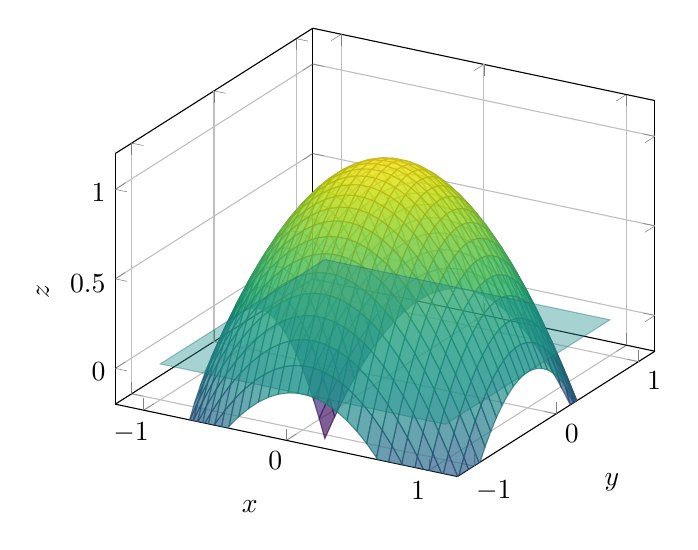
\begin{tikzpicture}
\begin{axis}[
    view={30}{30},
    xlabel=$x$, ylabel=$y$, zlabel=$z$,
    xmin=-1.2, xmax=1.2,
    ymin=-1.2, ymax=1.2,
    zmin=-0.2, zmax=1.2,
    colormap/viridis,
    grid=major
]
    % Paraboloid z = 1 - x^2 - y^2
    \addplot3[surf, domain=-1:1, y domain=-1:1, samples=30, opacity=0.7] {1 - x^2 - y^2};
    
    % Base plane z = 0 (Disk x^2 + y^2 <= 1)
    \addplot3[surf, domain=-1:1, y domain=-1:1, samples=2, opacity=0.4] {0};
    % Note: The domain of the plane is better handled by a disk, but a square suffices for visualization.
\end{axis}
\end{tikzpicture}
\end{document}
